\section{Thí nghiệm với mô hình robot hai bánh vi sai trong không gian 2D}

% {\color{red} BỔ SUNG MỤC ĐÍCH THÍ NGHIỆM VÀO ĐÂY=> KIỂM TRA KHẢ NĂNG ĐÁP ỨNG CỦA HỆ THỐNG VỚI THAM SỐ ĐỘNG HỌC TRONG NỀN TẢNG THÍ NGHIỆM GIẢ LẬP MÔI TRƯỜNG VẬT LÝ. NÓI RÕ NỘI DUNG NÀY ĐƯỢC THỰC HIỆN MỚI SO VỚI BÀI BÁO}
Trong phần thí nghiệm này sẽ tiến hành kiểm tra đánh giá đáp ứng của hệ thống với tham số động học trong nền tảng thí nghiệm giả lập môi trường vật lý. Không còn là môi trường chất điểm với các cảm biến được cho là lý tưởng, lúc này Robot sẽ sử dụng các mô đun cảm biến cùng với sự ảnh hưởng, tác động của nhiễu giống với thực tế.

\subsection{Nền tảng thí nghiệm Webots}

Thí nghiệm được thực hiện trên nền tảng mô phỏng giả lập môi trường vật lý, có tên gọi là Webots. Webots \cite{10.1007/3-540-68686-X_24} là một trình mô phỏng rô bốt 3D mã nguồn mở và miễn phí cho đa nền tảng, một môi trường phát triển được sử dụng để mô hình hóa, lập trình và mô phỏng robot di động. Với Webots, người dùng có thể thiết kế các thiết lập robot phức tạp, với một hoặc một số robot tương tự hoặc khác nhau, trong một môi trường chung. Các thuộc tính của từng đối tượng, chẳng hạn như hình dạng, màu sắc, kết cấu, khối lượng, ma sát, v.v., được người dùng lựa chọn. Một lựa chọn lớn các cảm biến mô phỏng và bộ truyền động có sẵn để trang bị cho mỗi robot. Bộ điều khiển robot có thể được lập trình với IDE tích hợp hoặc với môi trường phát triển của bên thứ ba. Hành vi của robot có thể được kiểm tra trong thế giới thực tế. Các chương trình điều khiển có thể tùy ý được chuyển sang các robot thực có bán trên thị trường. Hiện tại, Webots có thể hỗ trợ trên nhiều hệ điều hành khác nhau và hỗ trợ nhiều ngôn ngữ như C++ và Python, Matlab,...Thông tin chi tiết xem thêm trong Phụ lục \ref{sec:webot}.


\subsection{Robot di động e-puck}

Trong các thí nghiệm, đồ án sử dụng nền tảng robot di động cho giáo dục có tên gọi E-Puck. Nó là một robot di động thu nhỏ ban đầu được phát triển tại EPFL cho mục đích giảng dạy của các nhà thiết kế của robot Khepera thành công. Mô hình bao gồm hỗ trợ cho các động cơ bánh xe vi sai (bộ mã hóa cũng được mô phỏng, dưới dạng cảm biến vị trí), các cảm biến màu đỏ hồng , giao tiếp Bluetooth (được mô hình sử dụng thiết bị phát/ máy thu) và mở rộng cảm biến mặt đất.Robot có đường kính 71 mm và chiều cao phụ thuộc vào các module mở rộng được kết nối. Các kết cấu cơ khí của robot đều được làm bằng nhựa để giảm giá thành. Cấu trúc của robot rất đơn giản, chỉ gồm 4 bộ phận: thân chính, vòng đèn và 2 bánh xe, tất cả đều được làm bằng nhựa. Hai động cơ được gắn đơn giản vào thân chính, với bánh xe gắn trực tiếp vào trục động cơ. Một số thông tin quan trọng về Robot E-puck được trình bầy trong Bảng \ref{tab:Scoverage}, thông tin chi tiết hơn có thể xem tại Phụ lục \ref{sec:epuck}.
\begin{table}[h]
\centering
\caption{Một số thông tin robot E-puck trong phần mềm mô phỏng}
\label{tab:Scoverage}
\begin{tabular}{|l|c|c|c|c|c|c|c|c|c|c|}
\hline
\textbf{Đường kính robot($mm$)}      & 71  \\ \hline
\textbf{Chiều cao ($mm$)} & 50        \\ \hline
\textbf{Bán kính bánh xe($mm$)}      & 20.5  \\ \hline
\textbf{Trọng lượng ($kg$)} & 0.16        \\ \hline
\textbf{Tốc độ tối đa khi tiến/ lùi ($m/s$)} & 0.25       \\ \hline
\textbf{Tốc độ góc tối đa ($rad/s$)} & 6.28       \\ \hline
\textbf{Khoảng cách giữa hai bánh xe (mm)} & 52       \\ \hline
\end{tabular}
\end{table}

Mô hình động học của robot e-puck có thể được mô tả như sau: 
 
\begin{figure}[H]
    \centering
    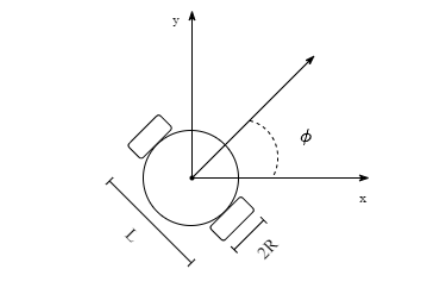
\includegraphics[scale=0.8]{chapter2/image/2banh.png}
    \caption{Mô hình robot 2 bánh vi sai}
    \label{fig:L298}
\end{figure}
Robot được coi là một chất điểm chuyển động trong đồ thị 2D dựa vào hệ quy
chiếu tọa độ và hướng, như vậy tọa độ của robot i được xác định bởi ba thành phần
$P(x,y,\theta)$ tốc độ $\overrightarrow{V}(x_{V},y_{V},\theta_{V})$ của robot i sẽ bằng vi phân tọa độ của P:
\begin{equation}
    \begin{aligned}
    \left\{ \begin{array}{c}
    x_{V}=\dfrac{\Delta x}{\Delta t}\\[1.5ex]
    y_{V}=\dfrac{\Delta y}{\Delta t}\\[1.5ex]
    \theta_{V}=\dfrac{\Delta\theta}{\Delta t}
    \end{array}\right.
    \end{aligned}
    \label{eqn:xytheta}
\end{equation}

Với mô hình robot được thiết kế hình tròn, hai động cơ được lắp đặt ở hai bên
giúp tâm robot nằm ở chính giữa. Với $\overrightarrow{V}(x_{V},y_{V},\theta_{V})$ là véc tơ vận tốc mong muốn của robot, chúng ta có thể sử dụng một mô hình động học dành cho robot hai bánh vi sai.
Vận tốc bánh trái $\omega_{L}$ là bánh phải $\omega_{R}$ được tính như sau:
\begin{equation}
    \begin{aligned}
        \left\{ \begin{array}{c}
        \omega_{L}=|\overrightarrow{V|}-\zeta*\dfrac{\theta_{t+1}-\theta_{t}}{\Delta_{t}}\\
        \omega_{R}=|\overrightarrow{V|}+\zeta*\dfrac{\theta_{t+1}-\theta_{t}}{\Delta_{t}}
        \end{array}\right.
    \end{aligned}
    \label{eqn:wlwr}
\end{equation}

Với hằng số $\zeta$ là hệ số điều chỉnh cố định, $\theta_{t+1}$ và $ \theta_{t}$
là góc giữa hướng của robot
và trục 0y tại thời điểm t + 1 và t


\subsection{Thực nghiệm trên Webots}

Ở các phần trước, trình bày quá trình tạo quỹ đạo đường đi cũng như là quá trình robot di chuyển trong quỹ đạo . Tuy nhiên robot chỉ là một chất điểm, chưa thực sự gắn lên trên mô hình robot thật với các thông số động học cụ thể. Do vậy ở phần thực nghiệm này sẽ được đưa vào bên trong một robot thật nhằm mục đích chỉ ra rằng bài toán này có thể áp dụng được vào trong thực tế. Robot có hệ thống cảm biến nhìn đa hướng, camera dạng toàn phương, có thể bao phủ một vùng nhất định xung quanh nó.

Trong phần này, quy trình tạo quỹ đạo cho robot không được thực hiện lại nữa, mà sẽ đánh giá quá trình hình thành đội hình chữ V và quá trình di chuyển thực hiện nhiệm vụ bao phủ của các robot. Robot được sử dụng là E-puck với việc trình bày thông số chi tiết động học ở bên trên như một robot ngoài đời với khả năng mô phỏng mạnh mẽ thể hiện trên trình mô phỏng vật lý Webots. Trình mô phỏng thực tế sẽ cho biết quá trình di chuyển của robot có bám sát theo quỹ đạo được tạo ra hay không, vùng thực tế bao phủ sẽ như thế nào khi đưa vào robot thật.

Đầu tiên, quá trình xây dựng bản đồ được thực hiện để phục vụ cho các thử nghiệm. Quy trình xây dựng môi trường sẽ được miêu tả kĩ ở Phụ lục \ref{sec:sim}. Môi trường của robot được thiết kế trên Webots, là một khu vực rộng lớn được bao phủ bởi 4 bức tường với các vật cản tĩnh như Hình \ref{fig:5Robot}.Các thông số của khu vực muốn bao phủ sẽ được thiết lập với từng hình dạng kích thước khác nhau tùy ý để đưa ra một quỹ đạo bao phủ cho robot Leader. Các robot sẽ được sắp xếp ngẫu nhiên các vị trí khác nhau sau đó chúng sẽ di chuyển dần dần lại để tạo ra hình dạng chữ V mong muốn. Các robot sẽ khảo sát trên khu vực polygon hình ngũ giác với 5 điểm mốc (x,y) lần lượt là: (174, -120), (-38, -156), (-124, 48), (-62, 122), (104, 52).


\begin{figure}[H]
    \centering
    \includegraphics[width=0.9\textwidth]{chapter5/image/Webot.png}
    \caption{Đội hình 5 robot trong Webots}
    \label{fig:5Robot}
\end{figure}


Quá trình hình thành đội hình được chỉ ra ở Hình \ref{fig:Vformation} . Robot leader sẽ bắt đầu di chuyển đồng thời tạo ra các điểm mốc ảo cho các follower. Do vị trí bắt đầu được sắp xếp ngẫu nhiên nên trong quá trình tiến đến các điểm ảo, các followers trong bầy phải chủ động tránh nhau, và dần dần hình thành lên cấu trúc chữ V mong muốn.


\begin{figure}[h!]
    \centering
    \begin{subfigure}[b]{0.48\textwidth}
    \centering
    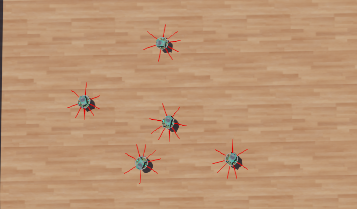
\includegraphics[width=\textwidth]{chapter5/image/buoc0.png}
    \caption{}
    \end{subfigure}
    \begin{subfigure}[b]{0.48\textwidth}
    \centering
    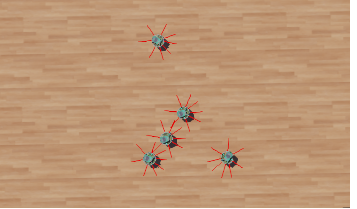
\includegraphics[width=\textwidth]{chapter5/image/buoc2.png}
    \caption{}
    \end{subfigure}
    \begin{subfigure}[b]{0.48\textwidth}
    \centering
    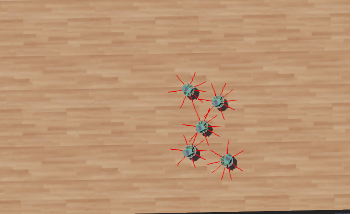
\includegraphics[width=\textwidth]{chapter5/image/buoc1.png}
    \caption{}
    \end{subfigure}
    \begin{subfigure}[b]{0.48\textwidth}
    \centering
    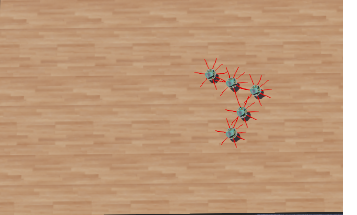
\includegraphics[width=\textwidth]{chapter5/image/buoc3.png}
    \caption{}
    \end{subfigure}
    \caption{Hình thành đội hình chữ V}
    \label{fig:Vformation}
\end{figure}

\begin{figure}[h!]
    \centering
    \begin{subfigure}[b]{0.49\textwidth}
    \centering
    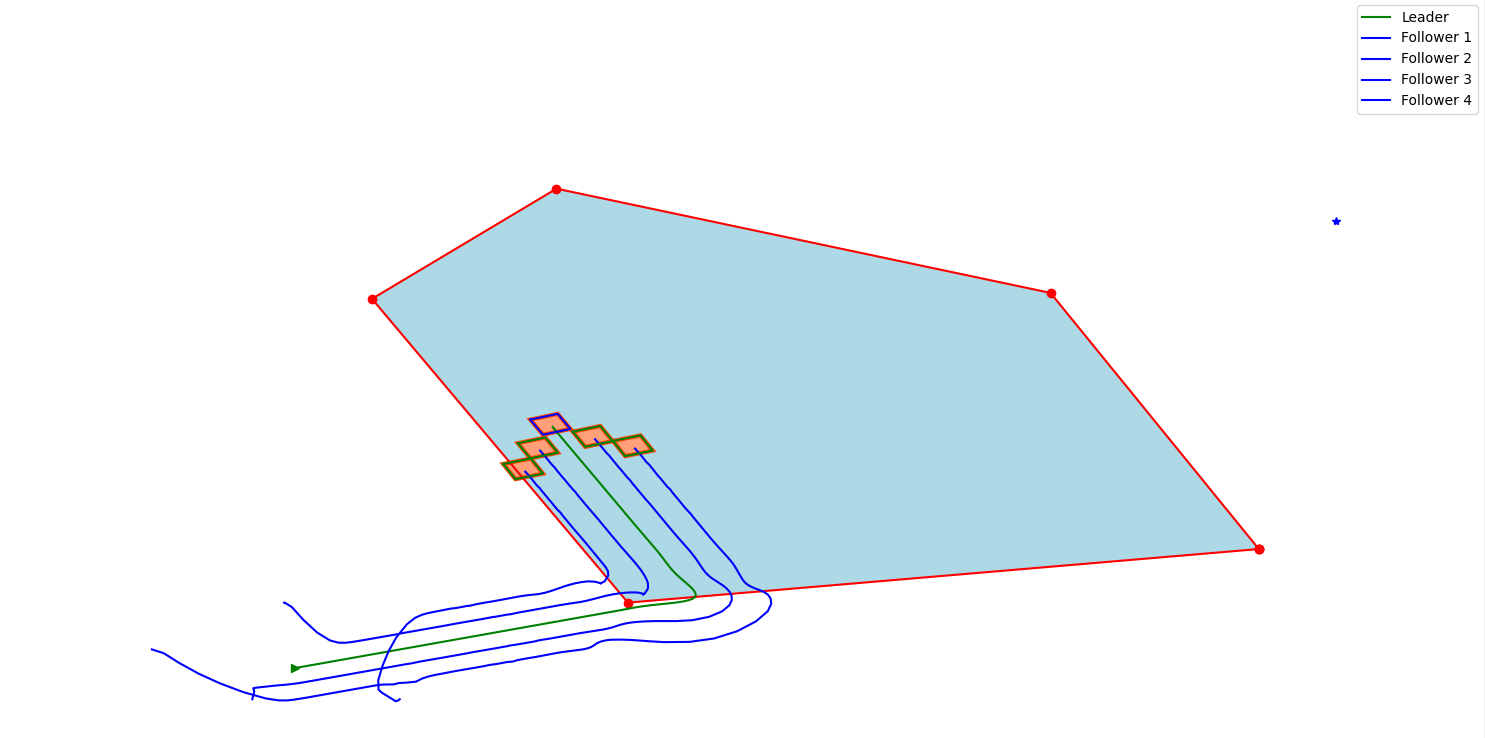
\includegraphics[width=\textwidth]{chapter5/image/quydao.png}
    \caption{}
    \end{subfigure}
    \begin{subfigure}[b]{0.49\textwidth}
    \centering
    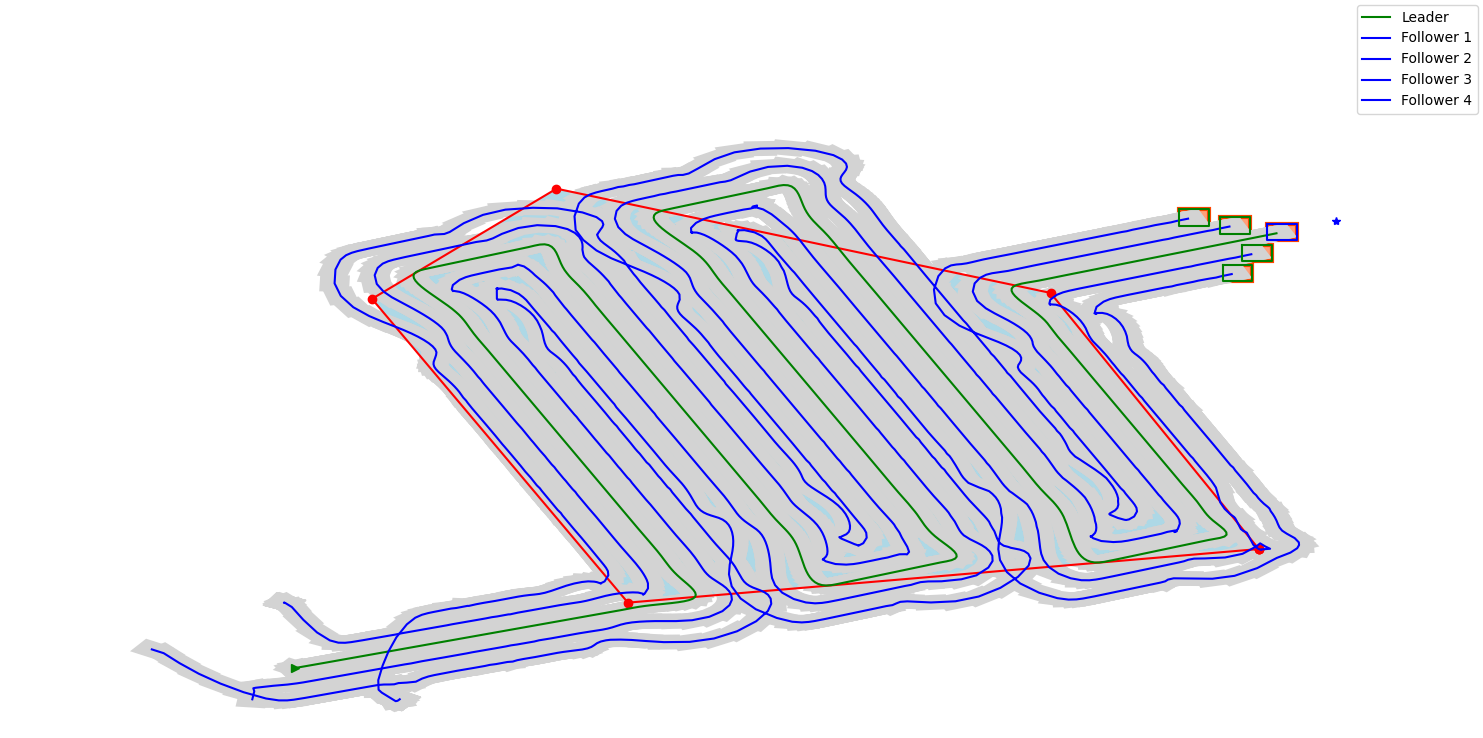
\includegraphics[width=\textwidth]{chapter5/image/rate.png}
    \caption{}
    \end{subfigure}
    \caption{Quá trình bao phủ của robot thực tế}
    \label{fig:noobs}
\end{figure}

\begin{figure}[H]
    \centering
    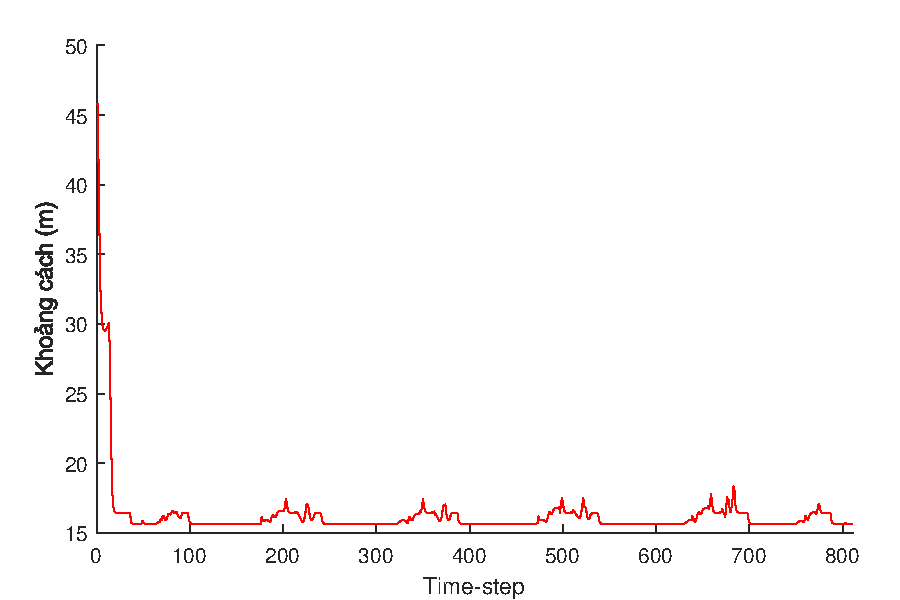
\includegraphics[width=0.65\textwidth]{chapter5/image/Median_Dis1.pdf}
    \caption{Trung vị khoảng cách 2 robot liên tiếp trong môi trường không vật cản}
    \label{fig:errdis}
\end{figure}

\begin{figure}[H]
    \centering
    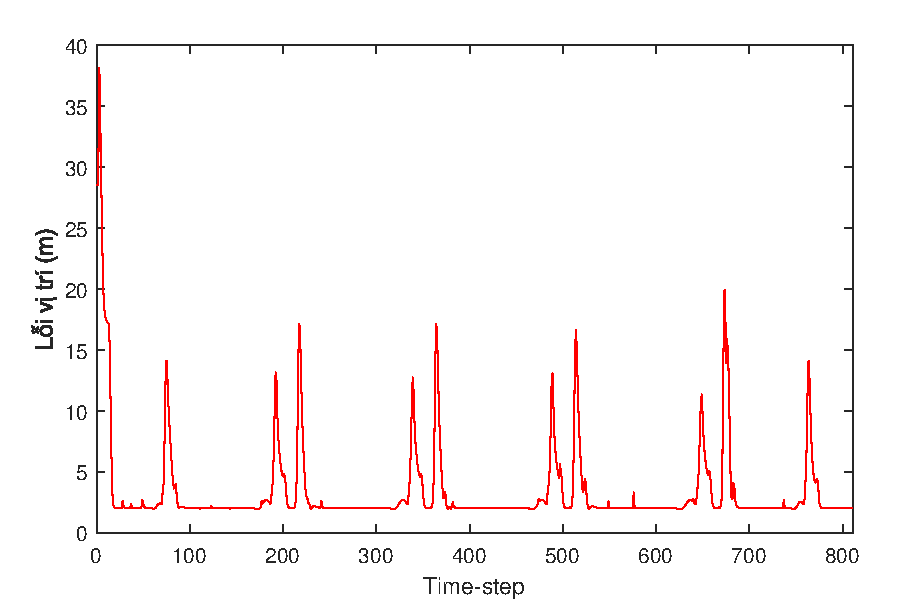
\includegraphics[width=0.65\textwidth]{chapter5/image/Median_Err1.pdf}
    \caption{Trung vị sai số vị trí vị trí follower và các điểm đích ảo trong môi trường không vật cản}
    \label{fig:errpos}
\end{figure}
Các robot tạo liên kết đội hình nhanh chóng trước khi bắt đầu vào khu vực để khảo sát. Quá trình mô phỏng thực tế vẫn đạt được độ bao phủ cao, cùng với sự ổn định của đội hình bay, mức độ bao phủ vẫn lên đến 96,7$\%$. Leader và các follower có quỹ đạo di chuyển bám sát với đường đi toàn cục tạo ra từ hệ thống. Thời gian xử lý trung bình cho mỗi bước tính toán là khoảng 0.03s.  Hình \ref{fig:errdis} và  \ref{fig:errpos} đồ thị cũng chỉ ra là giai đoạn đầu trung vị khoảng cách sai số của các con robot cạnh nhau và lỗi vị trí của robot với điểm đích ảo là rất lớn. Sau một khoảng thời gian ngắn bầy robot đã dần ổn định vị trí và hình thành nên đội hình chữ V. Ngoài ra, cũng giống như ở môi trường chất điểm, đối với những đoạn đường zig zag, leader di chuyển nhanh đột ngột, việc đội hình bị mất ổn định vẫn xảy ra. Tuy nhiên do có các thông số về động học, hành vi giữ đội hình đã thể hiện được đúng ý nghĩa hơn. Quỹ đạo ở khúc cua của robot follower cong và không xuất hiện những quỹ đạo khiến follower phải quay đầu như hình \ref{fig:2}. 

\textbf{Thực nghiệm trong môi trường có vật cản}:

\begin{figure}[H]
    \centering
    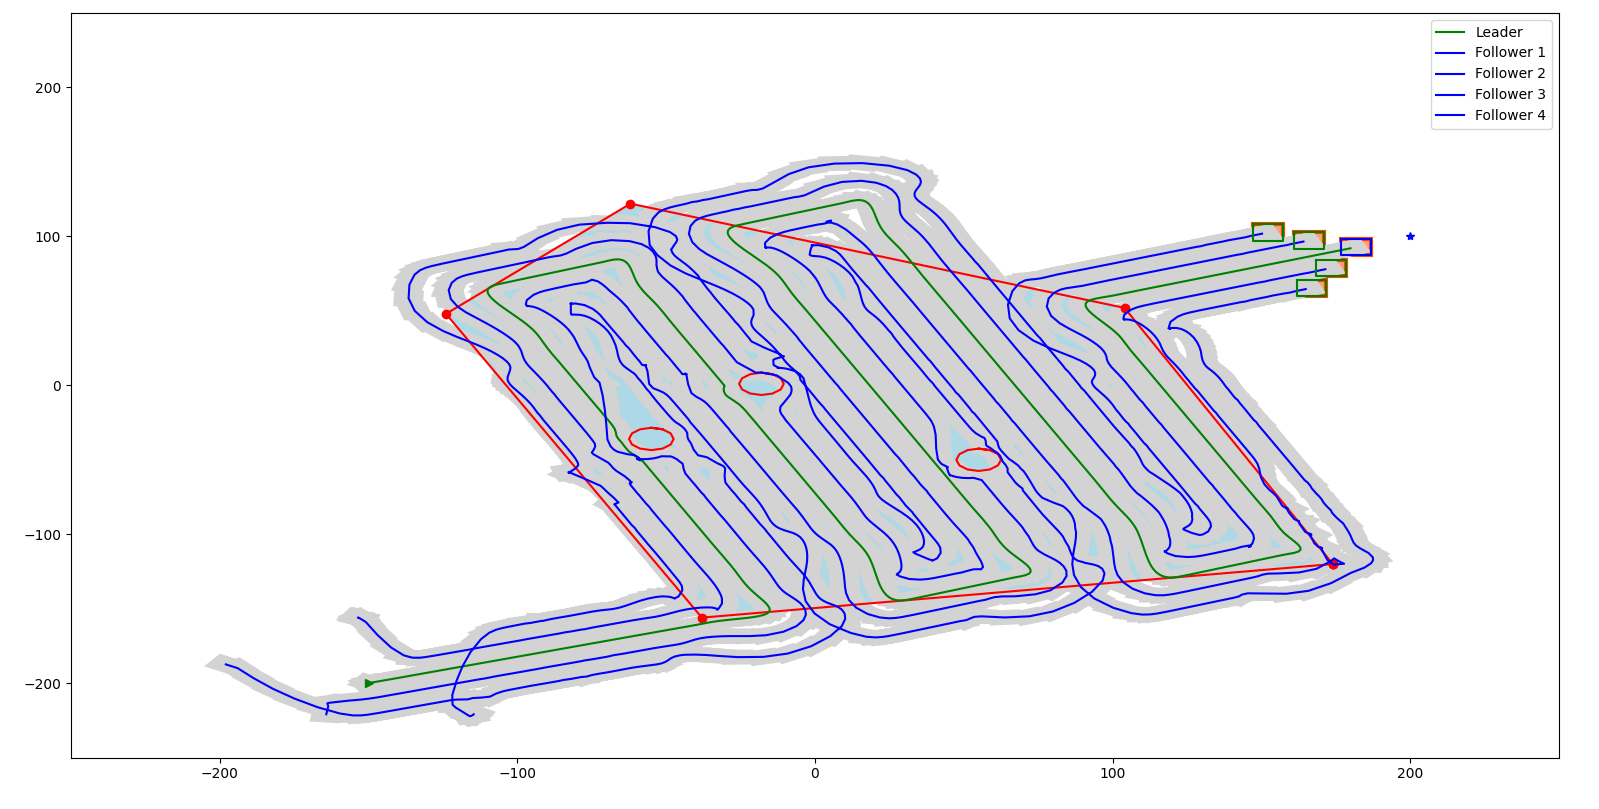
\includegraphics[width=0.9\textwidth]{chapter5/image/rateobs.png}
    \caption{Quỹ đạo bao phủ của bầy robot trong môi trường vật cản tĩnh}
    \label{fig:rateobs}
\end{figure}

\begin{figure}[H]
    \centering
    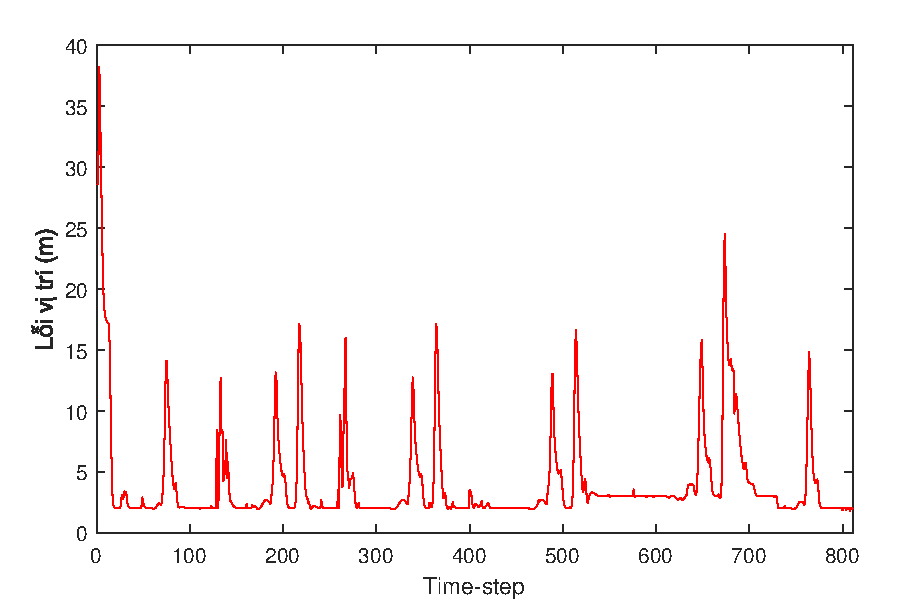
\includegraphics[width=0.75\textwidth]{chapter5/image/Median_Err2.pdf}
    \caption{Trung vị sai số vị trí vị trí follower và các điểm đích ảo trong môi trường vật cản tĩnh}
    \label{fig:med_errpos}
\end{figure}

\begin{figure}[H]
    \centering
    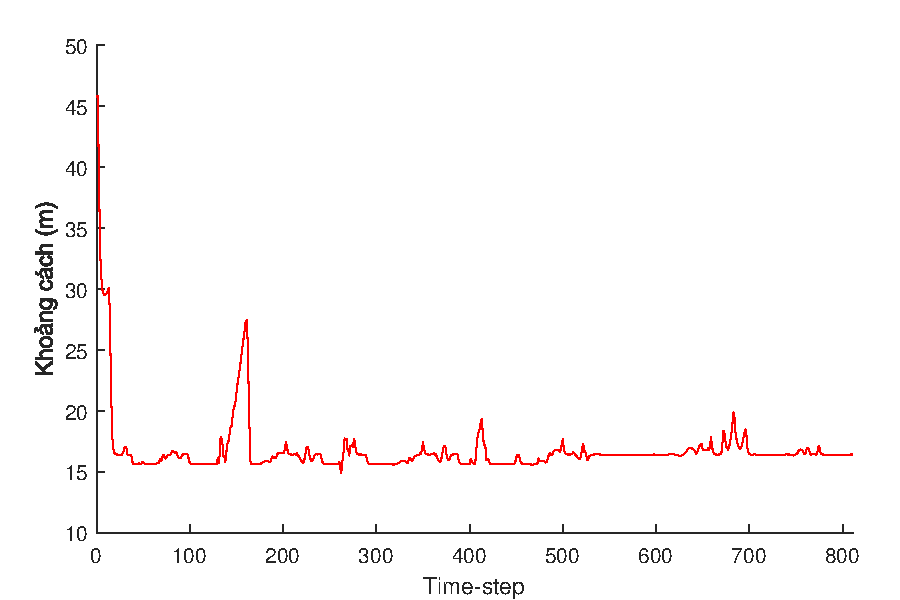
\includegraphics[width=0.75\textwidth]{chapter5/image/Median_Dis2.pdf}
    \caption{Trung vị khoảng cách 2 robot liên tiếp trong môi trường vật cản tĩnh}
    \label{fig:med_errdis}
\end{figure}

Trong hình \ref{fig:rateobs} chỉ ra quỹ đạo của robot Epuck trong quá trình tránh vật cản tĩnh. Về cơ bản robot đã né được vật cản. Tuy nhiên hành vi này cũng dẫn đến việc robot không thể bao phủ được những vùng xung quanh gần vật cản. Kết quả thu được phần diện tích bao phủ vẫn duy trì ở mức 93.55 $\%$ . Ngoài ra, Hình.\ref{fig:med_errdis} chỉ ra rằng mức độ ổn định của đội hình robot trong quá trình di chuyển. Qua đó thấy rằng khi đội hình Robot di chuyển trên đoạn đường thẳng, giá trị trung vị khoảng cách tương đối giữa hai robot liên tiếp luôn được duy trì ở mức ổn định. Trong trường hợp này đội hình liên tục phải di chuyển gặp vật cản cũng như các khúc rẽ nên có sai số dao động liên tục trong với độ lệch chuẩn là  $3.2\%$-$18.34\%$. Đối với lỗi vị trí trong Hình \ref{fig:med_errpos}, cũng như tổng khoảng cách vị trí hiện tại của các followers với các điểm vị trí ảo do leader tạo ra, đường đi thẳng có giá trị trung vị của các vị trí lỗi từ $2.5 m$ đến $16.5m $  khi nó giao động mạnh ở các khúc rẽ và khi gặp chưỡng ngại vật dẫn đến việc leader đổi hướng nhanh, hay đội hình bị phá vỡ khi các robot phải ưu tiên tránh vật cản. Tuy nhiên, nhờ vào hành vi duy trì đội hình được chỉ ra trong chương 2, đội hình chữ V dần dần quay lại trạng thái ổn định. Video kết quả quá trình di chuyển \footnote{\url{https://youtu.be/A5u8xT-GqYQ}}, 
\footnote{\url{https://youtu.be/n3JmeV05siU}}

 Nhìn chung với sự kết hợp đội hình cùng với việc sử dụng thuật toán tìm đường đi tối ưu có thể áp dụng triển khai trong mô phỏng với các cấu hình phần cứng được trình bày ở trên. Với khả năng theo sát được quỹ đạo đã tạo ra, thuật toán sẽ có tính khả thi cao và hoạt động theo thời gian thực trong thực tế.


% {\color{red} BỔ SUNG CLIP THÍ NGHIỆM VỚI Webots. lưu ý trong quyển dùng thống nhất Webots hay Webots, có s hay không cần chính xác}